\chapter{Understanding AI and Today's Applications}
\label{ch:ai-landscape}

\epigraph{The real problem is not whether machines think but whether men do.}{B.F. Skinner}

The previous chapter explained generative AI---the breakthrough that made AI accessible to everyone. But generative AI sits atop a broader foundation. To use it well, you need to understand the landscape: what AI actually means, how it differs from traditional software, and where it already operates in your business (whether you realize it or not).

This chapter provides that foundation. Think of it as the map before the journey.

\section{The Many Meanings of ``AI''}

Every quarter, someone walks into a board meeting with a slide deck featuring ``AI-powered'' solutions. The term has been stretched to cover everything from spam filters to autonomous vehicles. This creates confusion---and confusion is expensive.

When a vendor says ``AI-powered,'' they might mean rule-based systems that follow explicit if-then logic (traditional software, not really AI in the modern sense), or machine learning systems that learn patterns from data to make predictions. They might mean deep learning, which uses neural networks to handle complex patterns in images and language. Or they might mean generative AI---systems that create new content like text, images, and audio.

These categories nest inside each other like Russian dolls. All generative AI uses deep learning, all deep learning is machine learning, and all machine learning falls under the broad umbrella of artificial intelligence. But the capabilities and business applications differ dramatically at each level.

For this book, we focus primarily on generative AI and its practical business applications, because that is where the immediate opportunities lie for most executives. When you hear about ChatGPT, Claude, Copilot, or similar tools at industry conferences, you are hearing about generative AI.

\begin{figure}[htbp]
\centering
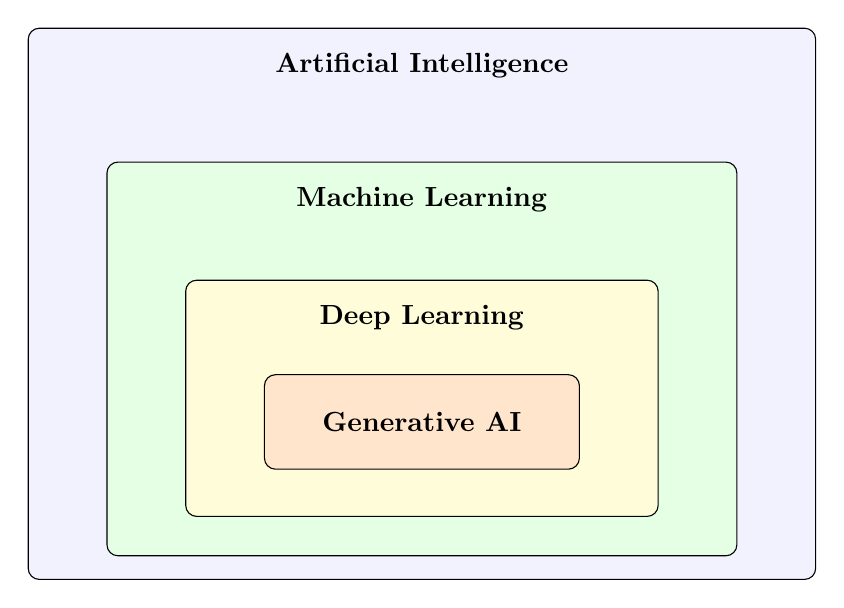
\begin{tikzpicture}
    % Outermost box - AI
    \node[draw, rounded corners, minimum width=10cm, minimum height=7cm, fill=blue!5] (ai) {};
    \node[anchor=north] at ([yshift=-0.2cm]ai.north) {\textbf{Artificial Intelligence}};

    % Machine Learning box
    \node[draw, rounded corners, minimum width=8cm, minimum height=5cm, fill=green!10] at ([yshift=-0.7cm]ai.center) (ml) {};
    \node[anchor=north] at ([yshift=-0.2cm]ml.north) {\textbf{Machine Learning}};

    % Deep Learning box
    \node[draw, rounded corners, minimum width=6cm, minimum height=3cm, fill=yellow!15] at ([yshift=-0.5cm]ml.center) (dl) {};
    \node[anchor=north] at ([yshift=-0.2cm]dl.north) {\textbf{Deep Learning}};

    % Generative AI box
    \node[draw, rounded corners, minimum width=4cm, minimum height=1.2cm, fill=orange!20] at ([yshift=-0.3cm]dl.center) (gen) {};
    \node at (gen.center) {\textbf{Generative AI}};
\end{tikzpicture}
\caption{The relationship between AI, machine learning, deep learning, and generative AI}
\label{fig:ai-hierarchy}
\end{figure}

\section{From Rules to Patterns: How AI Actually Works}

Understanding how predictive AI works helps you understand generative AI. Traditional business software follows explicit rules: ``If customer spent over \$1000, offer 10\% discount.'' Someone on your team wrote that rule, and the software executes it.

AI systems work differently. Instead of writing rules, you show the system thousands of examples: customers who responded well to various discounts, customers who did not. The system identifies patterns you never explicitly defined. Maybe it discovers that customers who browse on mobile devices on Sunday evenings respond better to free shipping than percentage discounts---an insight no analyst thought to formalize as a rule.

This shift from ``rules we write'' to ``patterns the system discovers'' is fundamental. Both predictive AI and generative AI rely on pattern discovery. The difference is what they do with those patterns. Predictive AI uses patterns to decide or classify (Does this look like fraud? Will this customer churn?). Generative AI uses patterns to produce (Write the next paragraph. Design a graphic. Generate a code snippet.)

\begin{table}[htbp]
\centering
\begin{tabularx}{\textwidth}{lXX}
\toprule
\textbf{Aspect} & \textbf{Traditional Software} & \textbf{AI Systems} \\
\midrule
Logic & Explicit rules written by humans & Patterns learned from examples \\
Updates & Requires code changes & Adapts with new data \\
Outputs & Deterministic, same input = same output & Probabilistic, may vary \\
Edge cases & Must be explicitly handled & May generalize or fail \\
Explainability & Clear, traceable logic & Often opaque (the ``black box'' problem) \\
\bottomrule
\end{tabularx}
\caption{Comparing traditional software and AI systems}
\end{table}

\section{What Generative AI Really Does}

Generative AI predicts what should come next.

When you ask ChatGPT a question, it is predicting: ``Given this question, what response would most likely follow based on billions of examples I learned from?'' It is not ``thinking'' or ``understanding'' in the human sense. It is sophisticated pattern matching at unprecedented scale.

This explains both its strengths and failures. It sounds fluent because it learned from fluent text. It can be confidently wrong because ``sounding right'' and ``being right'' are entirely different things. And it struggles with novel reasoning because it relies on patterns rather than genuine understanding.

\begin{keyinsight}
Think of generative AI as the world's most sophisticated autocomplete. It is remarkably good at predicting what text should come next based on patterns. But prediction is not understanding, and fluency is not accuracy. This distinction drives every decision about when to use AI and when to rely on human judgment.
\end{keyinsight}

\section{Where AI Is Already Around You}

Before you ``adopt AI,'' recognize you are already using it:

\begin{table}[htbp]
\centering
\begin{tabular}{ll}
\toprule
\textbf{Service} & \textbf{AI Application} \\
\midrule
Email spam filtering & Classification ML \\
Netflix recommendations & Recommendation systems \\
Google search results & Ranking algorithms + LLMs \\
Phone face unlock & Computer vision \\
Credit card fraud alerts & Anomaly detection \\
Autocorrect/autocomplete & Language models \\
\bottomrule
\end{tabular}
\caption{AI you already use daily}
\end{table}

The question is not whether to use AI---it is whether to use it more deliberately and strategically.

\section{The Business Case: Why Now?}

Previous AI hype cycles (2015, 2018) promised transformations that did not materialize for most businesses. Executives who ignored those waves often looked wise. This time is different, and here is why:

\textbf{Accessibility changed.} You no longer need a data science team to use AI. ChatGPT, Claude, and Copilot work through natural language. If you can describe what you want, you can use these tools. Your marketing director can use AI today---no IT ticket required.

\textbf{Capabilities crossed a threshold.} Pre-2022 language models were interesting but not business-ready. Current models can draft contracts, analyze financial reports, prepare board presentations, and summarize complex documents at a level that is genuinely useful.

\textbf{Cost dropped dramatically.} What cost thousands in computing three years ago now costs pennies per task. The unit economics changed fundamentally.

\textbf{The competitive pressure is real.} Your competitors are using these tools. The productivity gap between AI-assisted and non-AI-assisted work is widening. Early adopters are pulling ahead in operational efficiency.

\begin{realexample}[The Productivity Gap]
A professional services firm tracked two teams doing similar client analysis work. The team using AI tools consistently delivered reports 40\% faster with comparable quality. After six months, the difference in client capacity was significant. The AI-assisted team could handle more engagements, leading to higher revenue per consultant and better client satisfaction scores. The firm is now rolling out AI tools company-wide.
\end{realexample}

\section{What This Book Will and Will Not Cover}

This book focuses on practical application. You will learn how to use existing AI tools effectively---ChatGPT, Claude, Copilot, and specialized industry tools---along with frameworks for evaluating when AI is appropriate for a given task. We will cover managing AI risks around accuracy, privacy, and bias, implementing concrete projects with measurable results, and building organizational capability over time.

What we will not cover: building custom AI models from scratch, technical machine learning theory, AI for highly specialized domains like medical diagnosis or autonomous vehicles, or speculation about future capabilities that do not yet exist. This is a book about using AI as it exists today to solve business problems you face now.

\section{Summary}

AI is not one thing---it is a family of technologies, each with different capabilities and business applications. Machine learning finds patterns in data. Deep learning handles complex patterns like images and language. Generative AI creates new content based on those patterns.

You are already using AI, whether you realize it or not. The question is whether to use it more deliberately. The business case is stronger than ever: accessibility has increased, capabilities have crossed useful thresholds, costs have dropped, and competitive pressure is real.

With this foundation in place, the next chapter explores how AI systems actually ``think''---the mental models that explain both their remarkable capabilities and their surprising limitations.

\begin{exercise}
Identify three internal processes at your organization where generative AI could improve productivity. For each, outline: (1) what task the AI would perform, (2) how you would measure improvement, (3) what risks or concerns exist.
\end{exercise}

\begin{exercise}
Test ChatGPT, Claude, and Microsoft Copilot on the same prompts related to your industry. Document where they differ in quality, accuracy, and usefulness. What does this tell you about the current state of generative AI?
\end{exercise}
